\subsection{Lietotāja grafiskās saskarnes apraksts}
Programmas logs ir apskatāms \ref{fig:vessel-extractor} attēlā. Programma sastāv no vairākiem laukiem.  Datu vizualizācijas lauks ir paredzēts datortomogrāfijas slāņu vizualizācijai, kā arī asinsvadu tīklojuma 3D modeļa vizualizācijai. To, kas tiek attēlots var pārslēgt ar pogām: 2D View (Datortomogrāfija slāņu skats), 3D View (asinsvadu tīklojuma 3D modeļa skats). 3D modeļa skatā modelis ir aplūkojums tikai tad kad ir segmentēti asinsvadi, kā arī ģenerēts 3D modelis.
\begin{figure}[h]
\begin{center}
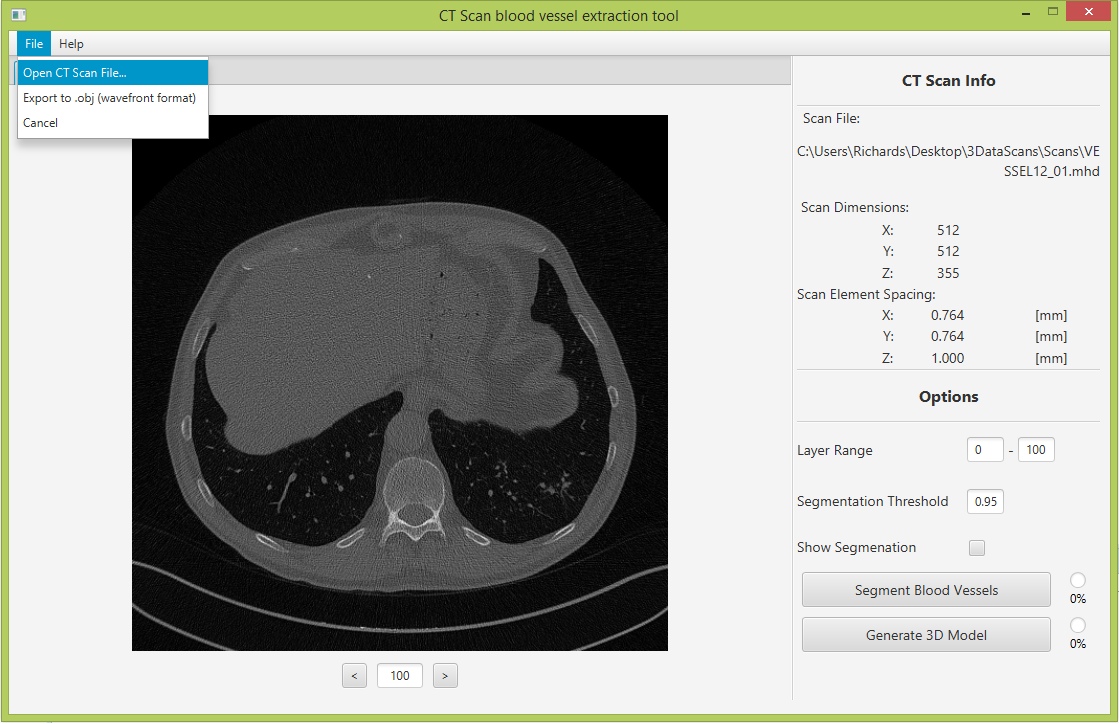
\includegraphics[scale=0.5]{img/vessel-extractor.png}
\caption{Asinsvadu segmentēšanas programmas logs}
\label{fig:vessel-extractor}
\end{center}
\end{figure}

